%%%%%%%%%%%%%%%%%%%%%%%%%%%%%%%%%%%%%%%%%
% Beamer Presentation
% LaTeX Template
% Version 1.0 (10/11/12)
%
% This template has been downloaded from:
% http://www.LaTeXTemplates.com
%
% License:
% CC BY-NC-SA 3.0 (http://creativecommons.org/licenses/by-nc-sa/3.0/)
%
%%%%%%%%%%%%%%%%%%%%%%%%%%%%%%%%%%%%%%%%%

%----------------------------------------------------------------------------------------
%	PACKAGES AND THEMES
%----------------------------------------------------------------------------------------

\documentclass{beamer}
\usepackage{mathtools}

\mode<presentation> {

% The Beamer class comes with a number of default slide themes
% which change the colors and layouts of slides. Below this is a list
% of all the themes, uncomment each in turn to see what they look like.

%\usetheme{default}
%\usetheme{AnnArbor}
%\usetheme{Antibes}
%\usetheme{Bergen}
%\usetheme{Berkeley}
%\usetheme{Berlin}
%\usetheme{Boadilla}
%\usetheme{CambridgeUS}
%\usetheme{Copenhagen}
%\usetheme{Darmstadt}
%\usetheme{Dresden}
%\usetheme{Frankfurt}
\usetheme{Goettingen}
%\usetheme{Hannover}
%\usetheme{Ilmenau}
%\usetheme{JuanLesPins}
%\usetheme{Luebeck}
%\usetheme{Madrid}
%\usetheme{Malmoe}
%\usetheme{Marburg}
%\usetheme{Montpellier}
%\usetheme{PaloAlto}
%\usetheme{Pittsburgh}
%\usetheme{Rochester}
%\usetheme{Singapore}
%\usetheme{Szeged}
%\usetheme{Warsaw}

% As well as themes, the Beamer class has a number of color themes
% for any slide theme. Uncomment each of these in turn to see how it
% changes the colors of your current slide theme.

%\usecolortheme{albatross}
%\usecolortheme{beaver}
%\usecolortheme{beetle}
%\usecolortheme{crane}
%\usecolortheme{dolphin}
%\usecolortheme{dove}
%\usecolortheme{fly}
%\usecolortheme{lily}
%\usecolortheme{orchid}
%\usecolortheme{rose}
%\usecolortheme{seagull}
%\usecolortheme{seahorse}
%\usecolortheme{whale}
%\usecolortheme{wolverine}

%\setbeamertemplate{footline} % To remove the footer line in all slides uncomment this line
%\setbeamertemplate{footline}[page number] % To replace the footer line in all slides with a simple slide count uncomment this line

%\setbeamertemplate{navigation symbols}{} % To remove the navigation symbols from the bottom of all slides uncomment this line
}

\usepackage{graphicx} % Allows including images
\usepackage{booktabs} % Allows the use of \toprule, \midrule and \bottomrule in tables

%----------------------------------------------------------------------------------------
%	TITLE PAGE
%----------------------------------------------------------------------------------------

\title[Superconductor Power Distr.]{Superconductor based Power Distribution} % The short title appears at the bottom of every slide, the full title is only on the title page

\author{Vinod, Joydeep, Biplob, Anita and Atul} % Your name
\institute[IISER M] % Your institution as it will appear on the bottom of every slide, may be shorthand to save space
{
Indian Institute of Science Education and Research Mohali \\ % Your institution for the title page
\medskip
% \textit{ms10024@iisermohali.ac.in} \\
% \textit{ms11003@iisermohali.ac.in} % Your email address
}
\date{\today} % Date, can be changed to a custom date

\begin{document}


\begin{frame}
\titlepage % Print the title page as the first slide
\end{frame}


\section{Outline}
\begin{frame}
\frametitle{Overview of the Talk} % Table of contents slide, comment this block out to remove it
\tableofcontents % Throughout your presentation, if you choose to use \section{} and \subsection{} commands, these will automatically be printed on this slide as an overview of your presentation
\end{frame}

\section{Prior Art}
	% \subsection{Motivation}
		\begin{frame}
			\frametitle{Current Scenario}
				\begin{figure}
					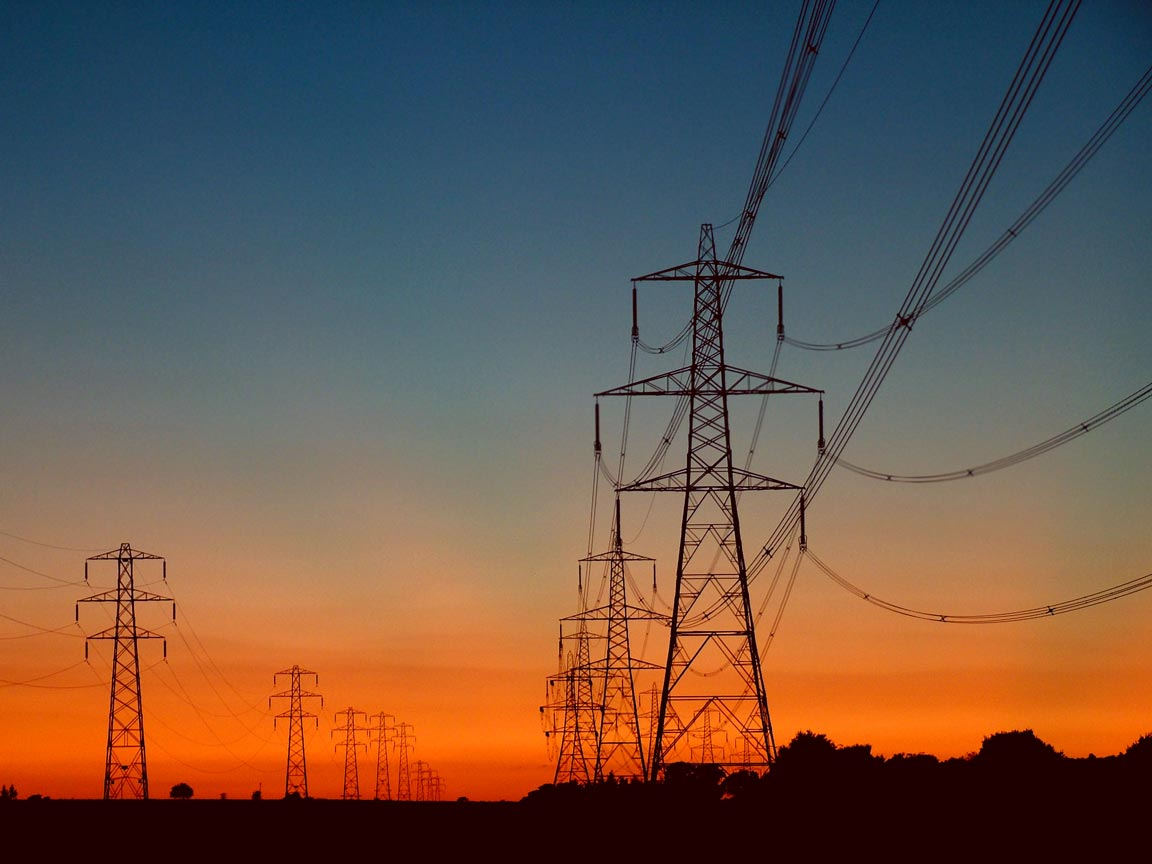
\includegraphics[width=0.8\linewidth]{powerlines}
				\end{figure}
		\end{frame}

	% \subsection{Superconductors}
		\begin{frame}
			\frametitle{Superconductor Description}
				\begin{itemize}
					\item Properties
					\item YBCO Wires [pictures follow]
						\begin{itemize}
							\item Manufacturing of YBCO
							\item Manufacture of Tape
							\item Manufacture of Wire
						\end{itemize}
					\item Cooling
						\begin{itemize}
							\item Running Temperature (~70 K)
							\item What happens when cooling fails | How the design helps
							\item Types of Losses
								\begin{itemize}
									\item Resistance (Joint losses)
									\item AC loss (magnetic losses)
								\end{itemize}
						\end{itemize}
				\end{itemize}
		\end{frame}

		\begin{frame}
			\begin{figure}
				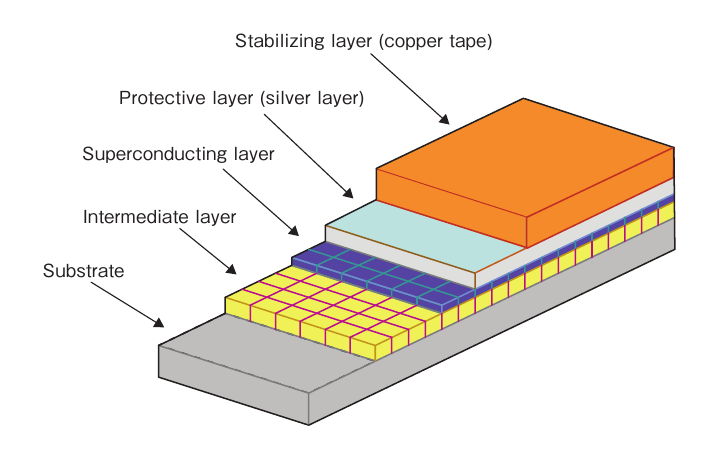
\includegraphics[width=0.9\linewidth]{YBCO}
				\caption[Structure of YBCO tape]{Structure of YBCO tape}
			\end{figure}
		\end{frame}

		\begin{frame}
			\begin{figure}
				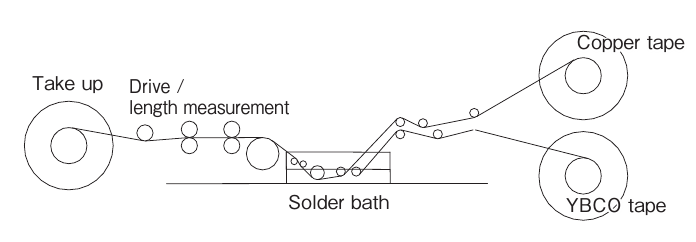
\includegraphics[width=0.9\linewidth]{laminating}
			\caption[Laminating machine for copper-composite YBCO tape]{Laminating machine for copper-composite YBCO tape}
			\end{figure}
		\end{frame}

		\begin{frame}
			\begin{figure}
				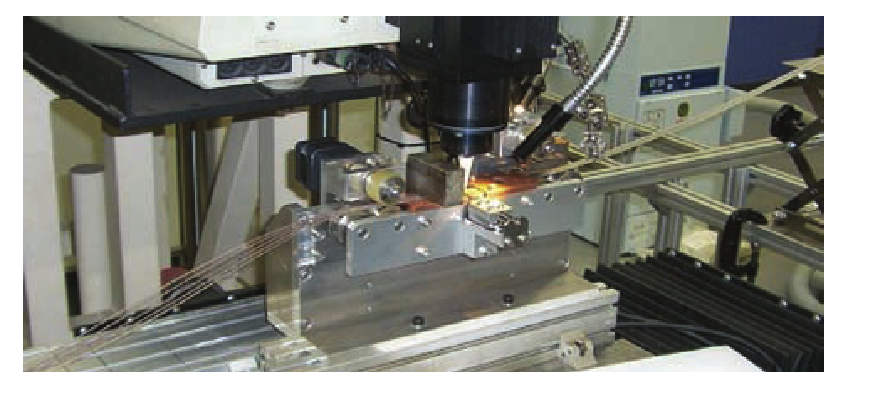
\includegraphics[width=0.9\linewidth]{lasercutting}
				\caption[Laser cutting machine for YBCO tapes]{Laser cutting machine for YBCO tapes}
			\end{figure}
		\end{frame}

		\begin{frame}
			\begin{figure}
				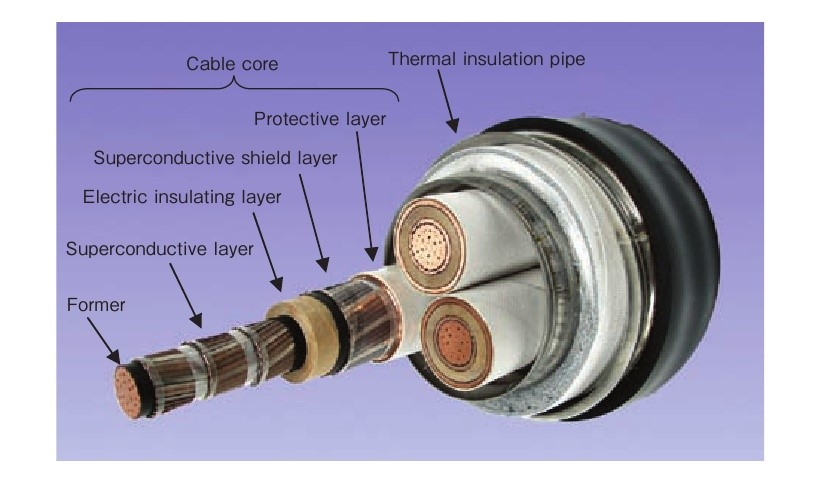
\includegraphics[width=0.9\linewidth]{3phase}
				\caption[HTS power cable]{HTS power cable}
			\end{figure}
		\end{frame}


		\begin{frame}
			\frametitle{AC DC}
				Losses
				\begin{itemize}
					\item Efficiency
						\begin{itemize}
							\item AC has both ohmic and AC loss (200 kW/km) [AC loss is dominant]
							\item DC has only ohmic (20 kW/km)
						\end{itemize}
					\item Number of wires
						\begin{itemize}
							\item For 3 phase AC, 4 wires required
							\item For DC, only 2 are required
						\end{itemize}
					% \item Cooling is easier						
				\end{itemize}
		\end{frame}

		\begin{frame}
			\frametitle{Status Quo}
				\begin{itemize}
					\item Power Generation [wikipedia page]
					\item Power Rate ~ 2.5 Rs / kWh
					\item Type of transmission | High voltage AC (500 KV), aluminium [550KV, 2500 $mm^2$, AC resistance 0.0168 $ohm/km$, reactance 0.199 $ohm/km$, max continuous current 1 kA]
				\end{itemize}
		\end{frame}


	% \subsection{}

\section{The Idea}
	
	\subsection{Smart Grid}
		\begin{frame}
			\frametitle{Smart Grid}
				Consider some state x, which has a power consumption of y MW and generates the same. If the generation fails, then power can be tapped from nearby states.\\
				It can distribute excess energy produced to the states that need it.\\				
				Power plants can now be placed without too many contrainsts on geographical locations.\\
				Further, power can be sold to nearby countries, should the generation exceed the demand.\\
				Power intensive projects can be setup without worrying about the location.\\
				\begin{itemize}					
					\item General advantage, if something fails, backup
					\item Easy distribution, to avoid wastes
					\item Location of powerplants
					\item Power can be sold
					\item Ease the setup of energy intensive projects
				\end{itemize}

		\end{frame}
	\subsection{Models}
		\begin{frame}
			\frametitle{Model for losses in Status Quo}
				\begin{itemize}
					\item State to state, connection
					\item Voltage: 500 KV
					\item Aluminium Wires [specified earlier]
					\item Number of wires, using max current rating
					\item Price per unit (KWh) [sepcified earlier]
					\item Power stations assumed in the capital
				\end{itemize}
		\end{frame}

		\begin{frame}
			\frametitle{Proposed Model}
				\begin{itemize}
					\item State to state, connection
					\item Voltages: 900 KV [Standard for scope for future development]\\
					Current capability: 70,000 A | max used: 36,111 A
					\item Calculations [will follow]
					\item Time for recovery ~ 
					\item Transformers for stepping up and stepping down 900 KV
					\item Distance from ground and distance between two wires
					\item Along highway
					\item Power station assumed in the capital
				\end{itemize}
		\end{frame}

	\subsection{The Calculations}
		\begin{frame}
			\frametitle{Algorithm/Formulae}
			Not considered
				\begin{itemize}
					\item Aluminium Wire laying cost
					\item Cooling cost (including maintenance)
					\item Islands
					\item AC/DC conversion losses
				\end{itemize}
			Discharge issues have been taken into account.\\
			The main idea has been summarized in the following equation.
		\end{frame}

		\begin{frame}
			\frametitle{The Cost Equation}
				\begin{equation}
					At = L^s_c + A^st
				\end{equation}
				where $A$ is the power loss in the current system, in Rupees per unit time,\\
				$L^s_c$ is the cost of installing the superconductor grid in Rupees,\\
				and $A^s$ is the running cost of the superconductor grid in Rupees, which has been assumed to be zero in accordance with the said assumptions.
		\end{frame}

	% \subsection{Laying Cost of Superdonductor}
		\begin{frame}
			\frametitle{Laying Cost of Superconductor $L^s_c$}
				$\$$: rate per unit distance (in Rupees, per meter, per 70,000A) \\
				$l$: Total Distance
				\begin{equation}
					L^s_c=2\$l
				\end{equation}
		\end{frame}
	
	% \subsection{Running Cost estimate of a similar conductor grid}
		\begin{frame}
			\frametitle{Running Cost estimate of a similar conductor grid $A$}
				\begin{equation}
					A=\sum_j(i_j^2R_j) C^{\text{Watt}}_{\text{Rs/t}}
				\end{equation}
				where $C^{\text{Watt}}_{\text{Rs/t}}$ is the conversion factor from Watt to Rs per unit time, the index $j$ counts uniquely, the connection between two cities, while the other variables have been defined as follows.\\
		\end{frame}

		\begin{frame}
			\frametitle{Running Cost estimate of a similar conductor grid $A$}
				Joule heating is given by $i_j^2R_jt$, where $i_j$ is the total current and $R_j$ the effective resistance of the wires joining the two cities.\\
				Given two cities\\
				$S_j \to l\equiv$ Distance between them\\
				$S_j \to p\equiv$ Max(Power produced by States)\\
				Thus,\\
				$i_j=\frac{S_j \to p}{V}$, where $V$ is the AC Voltage\\
				Further, $\#_{wires}=\lceil{\frac{S_j \to p}{i_wV}}\rceil$, where $i_w$ is the maximum current the wire can withstrand.\\
				And finally, we have $R_j=\frac{R_w}{\#_{wires}}S_j \to l$, where $R_w$ is the resistance of the wire per unit length.
				% Thus, finally\\
				% $R_j=\frac{R_w}{\#_{wires}}(S_j \to l)$.\\
				% Phew, that should do it.
		\end{frame}

		\begin{frame}	
			\frametitle{Calculations and Results}
				[Redirect to the excel sheet]
		\end{frame}

		\begin{frame}
			\frametitle{Summary of the result}
				From our estimates, installation cost of the superconductor grid would be recovered within 36.5 years, considering the current losses.
		\end{frame}

\section{Phases}
		\begin{frame}	
			\frametitle{Phase 1}
				Mini Test in IISER Mohali
				\begin{itemize}
					\item 10 m superconductor cable test.
					\item Wire cost ~ \$ 4,000
				\end{itemize}
		\end{frame}

		\begin{frame}	
			\frametitle{Phase 2}
				Test in IISER Mohali
				\begin{itemize}
					\item 500 m superconductor cable test.
					\item Wire cost ~ \$ 200,000
				\end{itemize}
		\end{frame}

		\begin{frame}
			\frametitle{Phase 3}
				Convincing the national funding agencies to accept the country wide grid's proposal
		\end{frame}

% {\del U}{\del n_1}
% %----------------------------------------------------------------------------------------
% %	PRESENTATION SLIDES
% %----------------------------------------------------------------------------------------

% %------------------------------------------------
% \section{First Section} % Sections can be created in order to organize your presentation into discrete blocks, all sections and subsections are automatically printed in the table of contents as an overview of the talk
% %------------------------------------------------

% \subsection{Subsection Example} % A subsection can be created just before a set of slides with a common theme to further break down your presentation into chunks

% \begin{frame}
% \frametitle{Paragraphs of Text}
% Sed iaculis dapibus gravida. Morbi sed tortor erat, nec interdum arcu. Sed id lorem lectus. Quisque viverra augue id sem ornare non aliquam nibh tristique. Aenean in ligula nisl. Nulla sed tellus ipsum. Donec vestibulum ligula non lorem vulputate fermentum accumsan neque mollis.\\~\\

% Sed diam enim, sagittis nec condimentum sit amet, ullamcorper sit amet libero. Aliquam vel dui orci, a porta odio. Nullam id suscipit ipsum. Aenean lobortis commodo sem, ut commodo leo gravida vitae. Pellentesque vehicula ante iaculis arcu pretium rutrum eget sit amet purus. Integer ornare nulla quis neque ultrices lobortis. Vestibulum ultrices tincidunt libero, quis commodo erat ullamcorper id.
% \end{frame}

% %------------------------------------------------

% \begin{frame}
% \frametitle{Bullet Points}
% \begin{itemize}
% \item Lorem ipsum dolor sit amet, consectetur adipiscing elit
% \item Aliquam blandit faucibus nisi, sit amet dapibus enim tempus eu
% \item Nulla commodo, erat quis gravida posuere, elit lacus lobortis est, quis porttitor odio mauris at libero
% \item Nam cursus est eget velit posuere pellentesque
% \item Vestibulum faucibus velit a augue condimentum quis convallis nulla gravida
% \end{itemize}
% \end{frame}

% %------------------------------------------------

% \begin{frame}
% \frametitle{Blocks of Highlighted Text}
% \begin{block}{Block 1}
% Lorem ipsum dolor sit amet, consectetur adipiscing elit. Integer lectus nisl, ultricies in feugiat rutrum, porttitor sit amet augue. Aliquam ut tortor mauris. Sed volutpat ante purus, quis accumsan dolor.
% \end{block}

% \begin{block}{Block 2}
% Pellentesque sed tellus purus. Class aptent taciti sociosqu ad litora torquent per conubia nostra, per inceptos himenaeos. Vestibulum quis magna at risus dictum tempor eu vitae velit.
% \end{block}

% \begin{block}{Block 3}
% Suspendisse tincidunt sagittis gravida. Curabitur condimentum, enim sed venenatis rutrum, ipsum neque consectetur orci, sed blandit justo nisi ac lacus.
% \end{block}
% \end{frame}

% %------------------------------------------------

% \begin{frame}
% \frametitle{Multiple Columns}
% \begin{columns}[c] % The "c" option specifies centered vertical alignment while the "t" option is used for top vertical alignment

% \column{.45\textwidth} % Left column and width
% \textbf{Heading}
% \begin{enumerate}
% \item Statement
% \item Explanation
% \item Example
% \end{enumerate}

% \column{.5\textwidth} % Right column and width
% Lorem ipsum dolor sit amet, consectetur adipiscing elit. Integer lectus nisl, ultricies in feugiat rutrum, porttitor sit amet augue. Aliquam ut tortor mauris. Sed volutpat ante purus, quis accumsan dolor.

% \end{columns}
% \end{frame}

% %------------------------------------------------
% \section{Second Section}
% %------------------------------------------------

% \begin{frame}
% \frametitle{Table}
% \begin{table}
% \begin{tabular}{l l l}
% \toprule
% \textbf{Treatments} & \textbf{Response 1} & \textbf{Response 2}\\
% \midrule
% Treatment 1 & 0.0003262 & 0.562 \\
% Treatment 2 & 0.0015681 & 0.910 \\
% Treatment 3 & 0.0009271 & 0.296 \\
% \bottomrule
% \end{tabular}
% \caption{Table caption}
% \end{table}
% \end{frame}

% %------------------------------------------------

% \begin{frame}
% \frametitle{Theorem}
% \begin{theorem}[Mass--energy equivalence]
% $E = mc^2$
% \end{theorem}
% \end{frame}

% %------------------------------------------------

% \begin{frame}[fragile] % Need to use the fragile option when verbatim is used in the slide
% \frametitle{Verbatim}
% \begin{example}[Theorem Slide Code]
% \begin{verbatim}
% \begin{frame}
% \frametitle{Theorem}
% \begin{theorem}[Mass--energy equivalence]
% $E = mc^2$
% \end{theorem}
% \end{frame}\end{verbatim}
% \end{example}
% \end{frame}

% %------------------------------------------------

% \begin{frame}
% \frametitle{Figure}
% Uncomment the code on this slide to include your own image from the same directory as the template .TeX file.
% %\begin{figure}
% %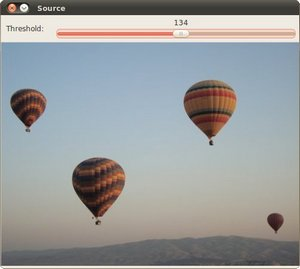
\includegraphics[width=0.8\linewidth]{test}
% %\end{figure}
% \end{frame}

% %------------------------------------------------

% \begin{frame}[fragile] % Need to use the fragile option when verbatim is used in the slide
% \frametitle{Citation}
% An example of the \verb|\cite| command to cite within the presentation:\\~

% This statement requires citation \cite{p1}.
% \end{frame}

% %------------------------------------------------

% \begin{frame}
% \frametitle{References}
% \footnotesize{
% \begin{thebibliography}{99} % Beamer does not support BibTeX so references must be inserted manually as below
% \bibitem[Smith, 2012]{p1} John Smith (2012)
% \newblock Title of the publication
% \newblock \emph{Journal Name} 12(3), 45 -- 678.
% \end{thebibliography}
% }
% \end{frame}

%------------------------------------------------
\section{References}
	\begin{frame}
	\frametitle{References}
		\begin{enumerate}
		\item M. HIROSE, T. MASUDA, K. SATO, R. HATA, High-Temperature Superconducting
		(HTS) DC Cable. \textbf{SEI TECHNICAL REVIEW 2006, 61, 29}. 
		\item S. Mukoyama, M. Yagi, H. Hirata, M. Suzuki, S. Nagaya, N.
		Kashima, Y. Shiohara, Development of YBCO High-Tc Superconducting
		Power Cables. \textbf{Furukawa Review 2009, 35}. 
		\item \href{http://www.forumofregulators.gov.in/data/study/capital-cost-branchmark.rk}{www.forumofregulators.gov.in/data/study/capital-cost-branchmark.rk}
		\item \href{http://www.bsesdelhi.com/HTML/wb-bsesatagiance.html }{www.bsesdelhi.com/HTML/wb-bsesatagiance.html }
		\item \href{http://www.wikipedia.com}{http://www.wikipedia.com}
		\end{enumerate}
	\end{frame}

\section{Closing Remarks}
	\begin{frame}
	\Huge{\centerline{Thank you}}
	\begin{figure}
		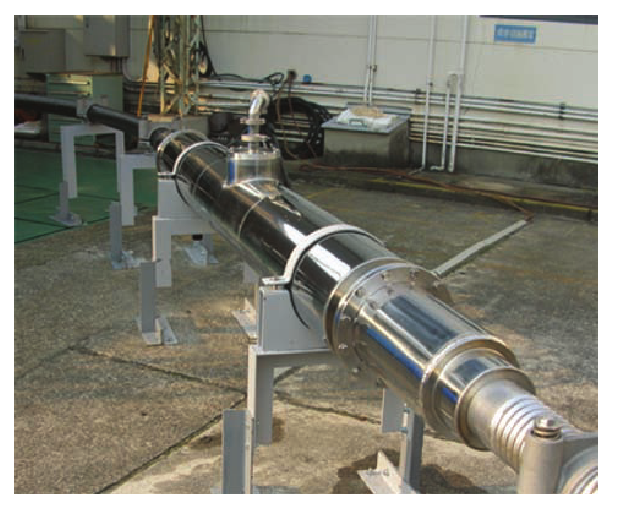
\includegraphics[width=0.8\linewidth]{normal}
	\end{figure}
	\end{frame}

%----------------------------------------------------------------------------------------

\end{document} 